\chapter{Electromagnetic Theory}
\begin{enumerate}
	\item  The electrostatic potential due to a charge distribution is given by
	$$
	V(r)=A \frac{e^{-\lambda r}}{r} \quad \text { where } A \text { and } \lambda \text { are constants. }
	$$
	The total charge enclosed within a sphere of radius $\frac{1}{\lambda}$, with its origin at $r=0$ is given by
	 \begin{tasks}(4)
		\task[\textbf{a.}] $\frac{8 \pi \varepsilon_{0} A}{e}$
		\task[\textbf{b.}]$\frac{4 \pi \varepsilon_{0} A}{e}$
		\task[\textbf{c.}]$\frac{6 \pi \varepsilon_{0} A}{\sqrt{e}}$
		\task[\textbf{d.}] 0
	\end{tasks}
\begin{answer}
	$$
	\begin{aligned}
	\because V(r)&=A \frac{e^{-\lambda r}}{r}\\
	\vec{E}&=-\vec{\nabla} V=-A\left[\frac{r e^{-\lambda r} \times(-\lambda)-e^{-\lambda r}}{r^{2}}\right] \hat{r}=\frac{A e^{-\lambda r}}{r^{2}}(1+\lambda r) \hat{r}\\
	Q_{e n c}&=\varepsilon_{0} \mid \int \vec{E} \cdot d \vec{a}=\varepsilon_{0} \int_{0}^{\pi} \int_{0}^{2 \pi} \frac{A e^{-\lambda r}}{r^{2}}(1+\lambda r) \hat{r} \cdot r^{2} \sin \theta d \theta d \phi \hat{r}=4 \pi \varepsilon_{0} A e^{-\lambda r}(1+\lambda r)\\
	\text { Thus  } &\text{total charge  enclosed within a sphere of radius}r=\frac{1}{\lambda} \text { is }\\
	Q_{e n c}&=4 \pi \varepsilon_{0} A e^{-\lambda \frac{1}{\lambda}}\left(1+\lambda \frac{1}{\lambda}\right)=\frac{8 \pi \varepsilon_{0} A}{e}
\end{aligned}
$$
So the correct answer is \textbf{Option (a)}
\end{answer}
\item  If the electrostatic potential in spherical polar coordinates is
$$
\phi(r)=\phi_{0} e^{-r / r_{0}}
$$
where $\phi_{0}$ and $r_{0}$ are constants, then the charge density at a distance $r=r_{0}$ will be	
 \begin{tasks}(4)
	\task[\textbf{a.}]$\frac{\varepsilon_{0} \phi_{0}}{e r_{0}^{2}}$
	\task[\textbf{b.}]$\frac{e \varepsilon_{0} \phi_{0}}{2 r_{0}^{2}}$
	\task[\textbf{c.}]$-\frac{\varepsilon_{0} \phi_{0}}{e r_{0}^{2}}$
	\task[\textbf{d.}] $-\frac{2 e \varepsilon_{0} \phi_{0}}{r_{0}^{2}}$
\end{tasks}	
\begin{answer}
	$$
	\begin{aligned}
	\because \nabla^{2} \phi&=-\frac{\rho}{\varepsilon_{0}} \Rightarrow \rho=-\varepsilon_{0}\left(\nabla^{2} \phi\right)\\
	\nabla^{2} \phi&=\frac{1}{r^{2}} \frac{\partial}{\partial r}\left(r^{2} \frac{\partial \phi}{\partial r}\right)=\frac{1}{r^{2}} \frac{\partial}{\partial r}\left(r^{2} \times-\frac{\phi_{0}}{r_{0}} e^{-r / r_{0}}\right)=-\frac{1}{r^{2}} \frac{\phi_{0}}{r_{0}} \frac{\partial}{\partial r}\left(r^{2} \times e^{-r / r_{0}}\right)\\&=-\frac{1}{r^{2}} \frac{\phi_{0}}{r_{0}}\left[r^{2} \times-\frac{1}{r_{0}} e^{-r / r_{0}}+2 r e^{-r / r_{0}}\right]\\
	\Rightarrow \nabla^{2} \phi&=-\frac{\phi_{0}}{r_{0}}\left[-\frac{1}{r_{0}} e^{-r / r_{0}}+\frac{2}{r} e^{-r / r_{0}}\right]\\
	\text { At a distance } r&=r_{0}, \quad \nabla^{2} \phi=-\frac{\phi_{0}}{r_{0}}\left[-\frac{1}{r_{0}} e^{-1}+\frac{2}{r_{0}} e^{-1}\right]=-\frac{\phi_{0}}{r_{0}^{2} e} \Rightarrow \rho=-\varepsilon_{0}\left(-\frac{\phi_{0}}{r_{0}^{2} e}\right)=\frac{\phi_{0} \varepsilon_{0}}{r_{0}^{2} e}
\end{aligned}
$$
So the correct answer is \textbf{Option (a)}
\end{answer}
\item  Two infinitely large sheets having charge densities $\sigma_{1}$ and $\sigma_{2}$ respectively $\left(\sigma_{1}>\sigma_{2}\right)$ are placed near each other separated by distance $d$ $A$ charge ' $Q$ ' is placed in between two plates such that there is no effect on charge distribution on plates. Now this charge is moved at an angle of $45^{\circ}$ with the horizontal towards plate having charge density $\sigma_{2}$ by distance $a^{\prime}(a<d)$. Find the work done by electric field in the process.
\begin{figure}[H]
	\centering
	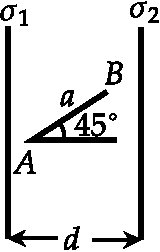
\includegraphics[height=3cm,width=2.2cm]{EMT-01}
\end{figure}
 \begin{tasks}(4)
	\task[\textbf{a.}]$\frac{q\left(\sigma_{1}-\sigma_{2}\right) a}{\varepsilon_{0}}$
	\task[\textbf{b.}]$\frac{q\left(\sigma_{1}-\sigma_{2}\right) a}{2 \varepsilon_{0}}$
	\task[\textbf{c.}] $\frac{q\left(\sigma_{1}-\sigma_{2}\right) a}{\sqrt{2} \varepsilon_{0}}$
	\task[\textbf{d.}] $\frac{q\left(\sigma_{1}-\sigma_{2}\right) a}{2 \sqrt{2} \varepsilon_{0}}$	
\end{tasks}	
\begin{answer}
	$$
	\begin{aligned}
	E&=\frac{\left(\sigma_{1}-\sigma_{2}\right)}{2 \varepsilon_{0}}\\ W&=\int \vec{F} \cdot d \vec{l}\\&=q E a \cos 45^{0}=q E \frac{a}{\sqrt{2}}\\&=\frac{q\left(\sigma_{1}-\sigma_{2}\right) a}{2 \sqrt{2} \varepsilon_{0}}
\end{aligned}
$$
So the correct answer is \textbf{Option (d)}
\end{answer}
\item  The electric fields outside $(r>R)$ and inside $(r<R)$ a solid sphere with a uniform volume charge density are given by $\vec{E}_{r>R}=\frac{1}{4 \pi \varepsilon_{0}} \frac{q}{r^{2}} \hat{r}$ and $\vec{E}_{r<R}=\frac{1}{4 \pi \varepsilon_{0}} \frac{q}{R^{3}} r \hat{r}$ respectively, while the electric field outside a spherical shell with a uniform surface charge density is given by	$\vec{E}_{r>R}=\frac{1}{4 \pi \varepsilon_{0}} \frac{q}{r^{2}} \hat{r}, q$ being the total charge. The correct ratio of the electrostatic energies for the second case to the first case is
 \begin{tasks}(4)
	\task[\textbf{a.}]$1: 3$
	\task[\textbf{b.}]$9: 16$
	\task[\textbf{c.}]$3: 8$
	\task[\textbf{d.}]$5: 6$ 
\end{tasks}	
\begin{answer}
	$$
	\begin{aligned}
	\text { Electrostatic energy in spherical shell } W_{s p}&=\frac{\in_{0}}{2} \int_{0}^{R}\left|\vec{E}_{1}\right|^{2} 4 \pi r^{2} d r+\frac{\in_{0}}{2} \int_{R}^{\infty}\left|\vec{E}_{2}\right|^{2} 4 \pi r^{2} d r\\
	\Rightarrow W_{s p}=\frac{\in_{0}}{2} \int_{R}^{\infty} \frac{q^{2}}{\left(4 \pi \in_{0}\right)^{2} r^{4}} 4 \pi r^{2} d r&=\frac{q^{2}}{8 \pi \in_{0}}\left(-\frac{1}{r}\right)_{R}^{\infty}=\frac{q^{2}}{8 \pi \in_{0}} \frac{1}{R}\\
	\text { Electrostatic energy in solid sphere } W_{s}&=\frac{\in_{0}}{2} \int_{0}^{R}\left|E_{1}\right|^{2} 4 \pi r^{2} d r+\frac{\in_{0}}{2} \int_{R}^{\infty}\left|E_{2}\right|^{2} 4 \pi r^{2} d r\\
	\Rightarrow W_{s}&=\frac{q^{2}}{8 \pi \in_{0}} \times \frac{1}{R^{6}}\left[\frac{r^{5}}{5}\right]_{0}^{R}+\frac{q^{2}}{8 \pi \in_{0}}\left[-\frac{1}{r}\right]_{R}^{\infty}\\
	\Rightarrow W_{s}&=\frac{q^{2}}{5 \times 8 \pi \epsilon_{0}} \cdot \frac{1}{R}+\frac{q^{2}}{8 \pi \epsilon_{0} R}=\frac{6 q^{2}}{40 \pi \epsilon_{0} R}\\
	Now
	\frac{W_{\text {spherical }}}{W_{\text {sphere }}}&=\frac{\frac{q^{2}}{8 \pi \epsilon_{0}}}{\frac{6 q^{2}}{40 \pi \epsilon_{0} R}}=\frac{5}{6}
\end{aligned}
$$
So the correct answer is \textbf{Option (d)}
\end{answer}
\item  Consider two concentric conducting spherical shells with inner and outer radii $a, b$ and $c, d$ as shown in the figure. Both the shells are given $q$ amount of positive charges. In order to have equal surface charge densities on the outer surface of both the shells, the following conditions should be satisfied	
\begin{figure}[H]
	\centering
	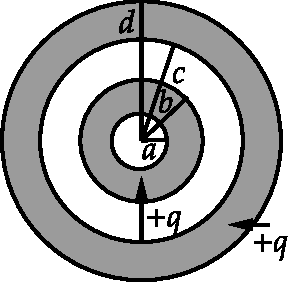
\includegraphics[height=3.5cm,width=3.6cm]{EMT-02}
\end{figure}
 \begin{tasks}(2)
	\task[\textbf{a.}]$d=4 b$ and $c=2 a$
	\task[\textbf{b.}]$d=2 b$ and $c=\sqrt{2} a$
	\task[\textbf{c.}]$d=\sqrt{2} b$ and $c>a$
	\task[\textbf{d.}] $d>b$ and $c=\sqrt{2} a$
\end{tasks}	
\begin{answer}
	$$
	\begin{aligned}
	\sigma_{b}&=\sigma_{d} \\ \frac{Q}{4 \pi b^{2}}&=\frac{2 Q}{4 \pi d^{2}} \\ d&=\sqrt{2} b
\end{aligned}
$$
So the correct answer is \textbf{Option (c)}
\end{answer}
\item  An ellipsoidal cavity is carved within a perfect conductor (figure). A Positive charge ' $q$ ' is placed at the center of the cavity. The points $A \& B$ are on the cavity surface as shown in figure. Then
\begin{figure}[H]
	\centering
	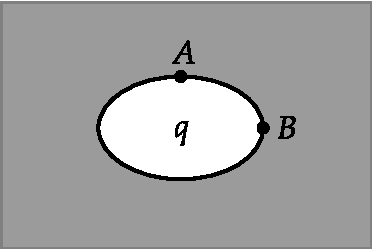
\includegraphics[height=3cm,width=5cm]{EMT-03}
\end{figure}	
 \begin{tasks}(1)
	\task[\textbf{a.}] Electric field near $A$ in the cavity $=$ electric field near $B$ in the cavity
	\task[\textbf{b.}]Charge density at $A=$ charge density at $B$
	\task[\textbf{c.}]Potential at $A=$ Potential at $B$
	\task[\textbf{d.}] Total electric flux through the surface of the cavity is $\frac{2 q}{\varepsilon_{0}}$	
\end{tasks}	
\begin{answer}
So the correct answer is \textbf{Option (c)}
\end{answer}
\item  A "pure" dipole with dipole moment $\vec{p}=p_{o} \hat{z}$ is situated at the origin. A point charge $Q$ is moved from the point $(a, 0,0)$ to $(0,0, a)$ then the work done will be
 \begin{tasks}(4)
	\task[\textbf{a.}]zero
	\task[\textbf{b.}] $\frac{p_{0} Q}{4 \pi \varepsilon_{0} a^{3}}$
	\task[\textbf{c.}]$\frac{p_{0}}{4 \pi \varepsilon_{0} a^{2}}$
	\task[\textbf{d.}] $\frac{p_{0} Q}{4 \pi \varepsilon_{0} a^{2}}$
\end{tasks}	
\begin{answer}
	$$
	\begin{aligned}
	W&=Q[V(0,0, a)-V(a, 0,0)]\\
	V(r, \theta)&=\frac{p_{0} \cos \theta}{4 \pi \varepsilon_{0} r^{2}} \Rightarrow V(0,0, a)=\frac{p_{0}}{4 \pi \varepsilon_{0} a^{2}} \quad \because \theta=0 \text { and } V(a, 0,0)=0 \quad \because \theta=\frac{\pi}{2}\\
	\Rightarrow W&=\frac{p_{0} Q}{4 \pi \varepsilon_{0} a^{2}}
\end{aligned}
$$
So the correct answer is \textbf{Option (d)}
\end{answer}
\item A point dipole with dipole moment $\vec{p}$ is oriented in the $z$-direction and located at the origin. The projection $E_{\perp}$ of the electric field strength vector (on the plane perpendicular to $\mathrm{Z}$-axis at the point $P$ ) is:	
\begin{figure}[H]
	\centering
	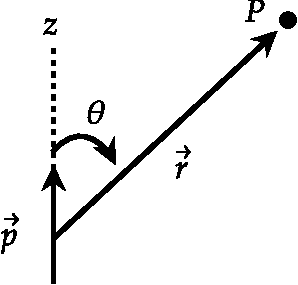
\includegraphics[height=3cm,width=3.5cm]{EMT-04}
\end{figure}	
 \begin{tasks}(2)
	\task[\textbf{a.}]$\frac{3 p \sin \theta \cos \theta}{4 \pi \varepsilon_{0} r^{3}}$
	\task[\textbf{b.}]$\frac{3 p \sin \theta}{4 \pi \varepsilon_{0} r^{3}}$
	\task[\textbf{c.}]$\frac{p}{4 \pi \varepsilon_{0} r^{3}}\left(3 \cos ^{2} \theta+1\right)$
	\task[\textbf{d.}]$\frac{p}{4 \pi \varepsilon_{0} r^{3}}\left(3 \cos ^{2} \theta-1\right)$
\end{tasks}	
\begin{answer}
	\begin{figure}[H]
		\centering
		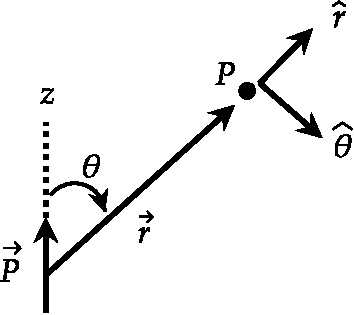
\includegraphics[height=3.5cm,width=4.5cm]{EMT-17}
	\end{figure}
	$$
	\begin{aligned}
	\vec{E}&=\frac{p}{4 \pi \varepsilon_{0} r^{3}}(2 \cos \theta \hat{r}+\sin \theta \hat{\theta}) \Rightarrow E_{r}=\frac{2 p \cos \theta}{4 \pi \varepsilon_{0} r^{3}} \text { and } E_{\theta}=\frac{p \sin \theta}{4 \pi \varepsilon_{0} r^{3}}\\
	E_{\perp}&=E_{r} \sin \theta+E_{\theta} \sin (90+\theta)\\
	\Rightarrow E_{\perp}&=E_{r} \sin \theta+E_{\theta} \cos \theta=\frac{2 p \cos \theta \sin \theta}{4 \pi \varepsilon_{0} r^{3}}+\frac{p \sin \theta \cos \theta}{4 \pi \varepsilon_{0} r^{3}}=\frac{3 p \sin \theta \cos \theta}{4 \pi \varepsilon_{0} r^{3}}
\end{aligned}
$$
So the correct answer is \textbf{Option (a)}
\end{answer}
\item  A point dipole with dipole moment $\vec{p}$ is oriented in the $z$-direction and located at the origin.
The angle $\theta$ at which $\vec{E}$ is perpendicular to $\vec{p}$ at point $P$ is
\begin{figure}[H]
	\centering
	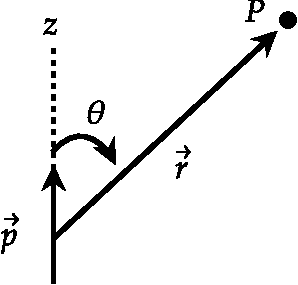
\includegraphics[height=3cm,width=3.5cm]{EMT-04}
\end{figure}
 \begin{tasks}(2)
	\task[\textbf{a.}]$\tan ^{-1}\left(\frac{1}{\sqrt{2}}\right)$
	\task[\textbf{b.}]$\tan ^{-1}(\sqrt{3})$
	\task[\textbf{c.}]$\sin ^{-1}\left(\frac{1}{\sqrt{3}}\right)$
	\task[\textbf{d.}] $\cos ^{-1}\left(\frac{1}{\sqrt{3}}\right)$	
\end{tasks}	
\begin{answer}$\left. \right. $\\
	\begin{figure}[H]
		\centering
		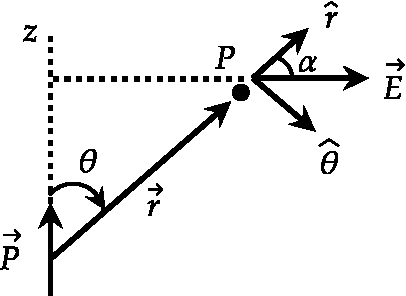
\includegraphics[height=3.2cm,width=5cm]{EMT-18}
	\end{figure}
	$$
	\begin{aligned}
	\vec{E}&=\frac{p}{4 \pi \varepsilon_{0} r^{3}}(2 \cos \theta \hat{r}+\sin \theta \hat{\theta}) \Rightarrow E_{r}=\frac{2 p \cos \theta}{4 \pi \varepsilon_{0} r^{3}} \text { and } E_{\theta}=\frac{p \sin \theta}{4 \pi \varepsilon_{0} r^{3}}\\
	\tan \alpha&=\frac{E_{\theta}}{E_{r}}=\frac{1}{2} \tan \theta\\
	\because \alpha&=90-\theta \Rightarrow \cot \theta=\frac{1}{2} \tan \theta \Rightarrow \tan ^{2} \theta=2 \Rightarrow \tan \theta=\sqrt{2}\\
	\Rightarrow \sin \theta&=\sqrt{\frac{2}{3}} \text { and } \cos \theta=\frac{1}{\sqrt{3}}
\end{aligned}
$$
So the correct answer is \textbf{Option (d)}
\end{answer}
\item  A dielectric sphere of radius $R$ has constant polarization $\vec{P}=P_{0} \hat{z}$ so that the field inside the sphere is $\vec{E}_{i n}=-\frac{P_{0}}{3 \varepsilon_{0}} \hat{z}$. Then, which of the following is not correct?
 \begin{tasks}(1)
	\task[\textbf{a.}]The bound surface charge density is $P_{0} \cos \theta$
	\task[\textbf{b.}]The electric field at a distance $r$ on the $z$ - axis varies as $\frac{1}{r^{2}}$ for $r>>$
	\task[\textbf{c.}]The electric potential at a distance $2 R$ on the $z$ - axis is $\frac{P_{0} R}{12 \varepsilon_{0}}$
	\task[\textbf{d.}] The electric field outside is equivalent to that of a dipole at the origin	
\end{tasks}	
\begin{answer}
	$$
	\begin{aligned}
	\sigma_{b}&=\vec{P} \cdot \hat{n}=\left(P_{0} \hat{z}\right) \cdot \hat{r}=P_{0} \cos \theta\\
	V_{d i p}&=\frac{1}{4 \pi \varepsilon_{0}} \frac{\vec{p} \cdot \hat{r}}{r^{2}}=\frac{1}{4 \pi \varepsilon_{0}} \frac{4 \pi R^{3}}{3} \frac{\vec{P} \cdot \hat{r}}{r^{2}}=\frac{1}{4 \pi \varepsilon_{0}} \frac{4 \pi R^{3}}{3} \frac{\left(P_{0} \hat{z}\right) . \hat{z}}{(2 R)^{2}}=\frac{P_{0} R}{12 \varepsilon_{0}}
\end{aligned}
$$
So the correct answer is \textbf{Option (b)}
\end{answer}
\item  A unit cube made of a dielectric material has a polarization $\vec{P}=3 \hat{i}+4 \hat{j}$ units. The edges of the cube are parallel to the Cartesian axes. Which of the following statement is true?	
 \begin{tasks}(1)
	\task[\textbf{a.}]The cube carries a volume bound charge of magnitude 5 units
	\task[\textbf{b.}]There is a charge of magnitude 3 units on both the surfaces parallel to the $y-z$ plane
	\task[\textbf{c.}]There is a charge of magnitude 5 units on both the surfaces parallel to the $x-z$ plane
	\task[\textbf{d.}] There is a net non-zero induced charge on the cube
\end{tasks}	
\begin{answer}
	$$
	\begin{aligned}
	\because \vec{P}&=3 \hat{i}+4 \hat{j} \Rightarrow \rho_{b}=-\vec{\nabla} \cdot \vec{P}=0 \text {. Option (a) is wrong }\\
	\text { At } x&=0, \sigma_{b}=\vec{P} \cdot \hat{n}=(3 \hat{i}+4 \hat{j}) \cdot(-\hat{i})=-3, \text { At } x=1, \sigma_{b}=\vec{P} \cdot \hat{n}=(3 \hat{i}+4 \hat{j}) \cdot(\hat{i})=3\\
	&\text { Option (b) is true }\\
	\text { At } y&=0, \sigma_{b}=\vec{P} \cdot \hat{n}=(3 \hat{i}+4 \hat{j}) \cdot(-\hat{j})=-4, \text { At } y=1, \sigma_{b}=\vec{P} \cdot \hat{n}=(3 \hat{i}+4 \hat{j}) \cdot(\hat{j})=4\\
&\text{	Option (c) is wrong.}\\
&\text{	Option (d) is wrong.}
\end{aligned}
$$
So the correct answer is \textbf{Option (b)}
\end{answer}
\item 	 Assume that $z=0$ plane is the interface between two linear and homogenous dielectrics (see figure). The relative permittivities are $\varepsilon_{r}=4$ for $z>0$ and $\varepsilon_{r}=5$ for $z<0$. The electric field in the region $z>0$ is $\vec{E}_{1}=(3 \hat{i}-5 \hat{j}+4 \hat{k}) k V / m$. If there are no free charges on the interface, then which of the following is true for the electric field in the region $z<0$ is given by
\begin{figure}[H]
	\centering
	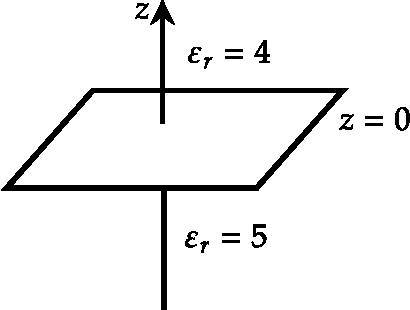
\includegraphics[height=3cm,width=5cm]{EMT-06}
\end{figure}
 \begin{tasks}(2)
	\task[\textbf{a.}]$\vec{E}_{2}=\left(3 \hat{i}-5 \hat{j}+\frac{16}{5} \hat{k}\right) k V / m$
	\task[\textbf{b.}]$\vec{E}_{2}=(-3 \hat{i}-5 \hat{j}-5 \hat{k}) k \quad V / m$	
	\task[\textbf{c.}]$\vec{E}_{2}=(3 \hat{i}-5 \hat{j}-5 \hat{k}) k V / m$
	\task[\textbf{d.}] $\vec{E}_{2}=(3 \hat{i}-5 \hat{j}+5 \hat{k}) k V / m$	
\end{tasks}	
\begin{answer}
	$$
	\begin{aligned}
	\because E_{1}^{\parallel}&=E_{2}^{\parallel} \Rightarrow E_{2}^{\parallel}=3 \hat{i}-5 \hat{j}\\
	\text { and } \sigma_{f}&=0 \Rightarrow D_{1}^{\perp}=D_{2}^{\perp} \Rightarrow E_{2}^{\perp}=\frac{\varepsilon_{1}}{\varepsilon_{2}} E_{1}^{\perp}=\frac{4}{5}(+4 \hat{k})=\frac{16}{5} \hat{k}\\
	\Rightarrow \vec{E}_{2}&=\left(3 \hat{i}-5 \hat{j}+\frac{16}{5} \hat{k}\right) k \quad V / m
\end{aligned}
$$
So the correct answer is \textbf{Option (a)}
\end{answer}
\item  Let four-point charges $q,-q / 2, q$ and $-q / 2$ be placed at the vertices of a square of side $a$. Let another point charge $-q$ be placed at the center of the square (see the figure).	
Let $E(r)$ be the electrostatic field at a point $P$ at a distance $r>>a$ from the centre of the square. Then $E(3 r) / E(2 r)$ is
\begin{figure}[H]
	\centering
	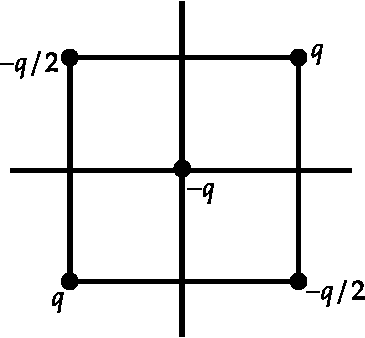
\includegraphics[height=3.7cm,width=4cm]{EMT-07}
\end{figure}
 \begin{tasks}(4)
	\task[\textbf{a.}]$\frac{1}{81}$
	\task[\textbf{b.}]$\frac{8}{27}$
	\task[\textbf{c.}]$\frac{4}{9}$
	\task[\textbf{d.}] $\frac{16}{81}$	
\end{tasks}
\begin{answer}
	$$
	\begin{aligned}
	\text { According to multipole expansion } Q_{\text {mono }}&=-\frac{q}{2}+q-\frac{q}{2}+q-q=0\\
	\vec{p}=q(a \hat{x}+a \hat{y})-\frac{q}{2}(a \hat{x}+a \hat{y})-q(a \hat{x}-a \hat{y})&+q(-a \hat{x}-a \hat{y})-\frac{q}{2}(-a \hat{x}+a \hat{y})+0=0\\
	\text { Thus } V \propto \frac{1}{r^{3}} \Rightarrow E \propto& \frac{1}{r^{4}} \Rightarrow \frac{E(3 r)}{E(2 r)}=\frac{16}{81}
\end{aligned}
$$
So the correct answer is \textbf{Option (d)}
\end{answer}
\item  Two charges $q$ and $3 q$ are placed along the $x$-axis in front of a grounded, infinite conducting plane, as shown in the figure. They are located respectively at a distance of $0.5 \mathrm{~m}$ and $1.5 \mathrm{~m}$ from the plane. The force acting on the charge $q$ is
(where $A$ is some constant and $x$ is variable distance)
\begin{figure}[H]
	\centering
	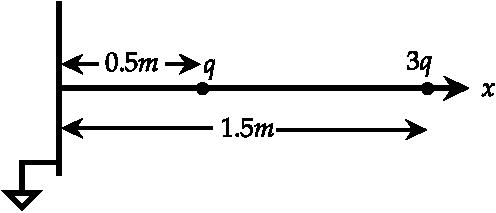
\includegraphics[height=2.5cm,width=6cm]{EMT-08}
\end{figure}
 \begin{tasks}(4)
	\task[\textbf{a.}] $\frac{1}{4 \pi \varepsilon_{0}} \frac{7 q^{2}}{2}$
	\task[\textbf{b.}]$\frac{1}{4 \pi \varepsilon_{0}} \frac{5 q^{2}}{4}$
	\task[\textbf{c.}]$\frac{1}{4 \pi \varepsilon_{0}} \frac{19 q^{2}}{4}$
	\task[\textbf{d.}] $\frac{1}{4 \pi \varepsilon_{0}} \frac{q^{2}}{2}$
\end{tasks}
\begin{answer}
	\text { Using method of Images we can draw equivalent figure as shown below: }
	\begin{figure}[H]
		\centering
		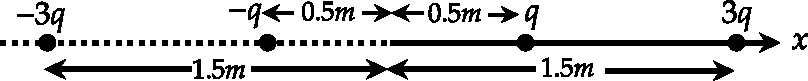
\includegraphics[height=1.1cm,width=10cm]{EMT-19}
	\end{figure}
	$$
	\begin{aligned}
	F=\frac{q}{4 \pi \varepsilon_{0}}\left[\frac{3 q}{(1)^{2}}+\frac{q}{(1)^{2}}+\frac{3 q}{(2)^{2}}\right]=\frac{q}{4 \pi \varepsilon_{0}} \times \frac{19 q}{4}=\frac{1}{4 \pi \varepsilon_{0}} \frac{19 q^{2}}{4}
\end{aligned}
$$
So the correct answer is \textbf{Option (c)}
\end{answer}
\item  A circular disc of radius $a$ on the $x y$ plane has a surface charge density $\sigma=\frac{\sigma_{0} r \cos \theta}{a}$. The electric dipole moment of this charge distribution is
 \begin{tasks}(2)
	\task[\textbf{a.}] $\frac{\sigma_{0} \pi a^{4}}{4} \hat{x}$
	\task[\textbf{b.}]$\frac{\sigma_{0} \pi a^{3}}{4} \hat{x}$
	\task[\textbf{c.}] $\frac{-\sigma_{0} \pi a^{3}}{4} \hat{x}$
	\task[\textbf{d.}]$\frac{-\sigma_{0} \pi a^{4}}{4} \hat{x}$ 
\end{tasks}
\begin{answer}
	$$
	\begin{aligned}
	\text { Dipole moment } \vec{p}&=\int \vec{r}^{\prime} \sigma\left(r^{\prime}\right) d a^{\prime}\\
	\text { Thus } p_{x}&=\int x^{\prime} \sigma\left(r^{\prime}\right) d a^{\prime}, p_{y}=\int y^{\prime} \sigma\left(r^{\prime}\right) d a^{\prime} \text { and } p_{z}=\int z^{\prime} \sigma\left(r^{\prime}\right) d a^{\prime} \text {. }\\
	p_{x}&=\iint(r \cos \theta) \times \frac{\sigma_{0} r \cos \theta}{a} d a^{\prime}=\int_{0}^{a} \int_{0}^{2 \pi} \frac{\sigma_{0} r^{2} \cos ^{2} \theta}{a} r d r d \theta\\
	p_{x}&=\frac{\sigma_{0}}{a} \int_{0}^{a} r^{3} d r \int_{0}^{2 \pi} \cos ^{2} \theta d \theta=\frac{\sigma_{0} a^{4}}{4 a} \times \pi=\frac{\sigma_{0} \pi a^{3}}{4} \Rightarrow \vec{p}=\frac{\sigma_{0} \pi a^{3}}{4} \hat{x}
\end{aligned}
$$
So the correct answer is \textbf{Option (b)}
\end{answer}


\end{enumerate}